\chapter{Introducción específica} % Main chapter title

\label{Chapter2}


%----------------------------------------------------------------------------------------
\section{Protocolos de comununicación utilizados}

  Comenzar escribiendo que aqui se detallaran los protocolos utilizados segun el modelo TCP/IP y hablar sobre el diagrama    

  AGREGAR UNA IMAGEN CON LOS 3 ENTES INTERCONECTADOS BAJO EL MODELO OSI 
        Nucleo F429ZI Board <----> Dedicated Server <----> Web Client


\subsection{Protocolos de comunicación}

De los modelos \textit{stack IoT} y \textit{lwIP} \citep{lwip}, basados en el stack \textit{TCP/IP} \footnote{\url{https://www.ibm.com/docs/en/aix/7.2?topic=protocol-tcpip-protocols}}, se emplean los siguientes protocolos de comunicación tal como se puede observar en la tabla \ref{tab:capa_protocolo}. 


\begin{table}[h]
\centering
\caption{Protocolos de comunicación utilizados en cada capa del \textit{stack TCP/IP}}
\label{tab:capa_protocolo}
\begin{tabular}{|c|c|}
\hline
\textbf{Capa} & \textbf{Protocolo} \\ \cline{1-2}
Capa de Aplicación & HTTP \citep{http}, DHCP \citep{dhcp} y MQTT \citep{mqtt} \\ \cline{1-2}
Capa de Transporte & UDP \citep{udp} \\ \cline{1-2}
Capa de Red & IPv4 \citep{ipv4}, ARP \citep{arp} \\ \cline{1-2}
Capa de Enlace de Datos & Ethernet \citep{ethernet} \\ \cline{1-2}
\end{tabular}
\end{table}

Cabe destacar que ambos modelos se encuentran diseñados para sistemas con recursos limitados y buscan garantizar una correcta comunicación entre los dispositivos conectados en la red.


%----------------------------------------------------------------------------------------
\section{Tecnologías \textit{full-stack}}

A partir de los modelos más relevantes que se encuentran establecidos para el desarrollo e implementación de aplicaciones de software se consideran el \textit{stack web} y el \textit{stack IoT}. A pesar de las similitudes entre ambos, en la aplicación el \textit{stack web} emplea el protocolo \textit{HTTP} mientras que el \textit{stack IoT} utiliza el protocolo \textit{MQTT}; siendo este último el más adecuado para escenarios donde son limitados los recursos como el ancho de banda y el consumo de energía.

En especial, el protocolo \textit{MQTT} dispone de mensajes más livianos y además es posible transmitir y/o recibir datos en formato binario sin la necesidad de una codificación previa. También, este protocolo permite asignar niveles de calidad de servicio (\textit{QoS} \footnote{\url{https://www.ibm.com/docs/en/i/7.2?topic=services-quality-service}}) a los mensajes transmitidos, resultando una característica primordial en aplicaciones donde la probabilidad de pérdidas de paquetes es considerable.

La figura 1 presenta la estratificación de las capas, según el \textit{stack IoT}, que son detalladas a lo largo de esta sección.

\begin{figure}[htpb]
  \centering 
  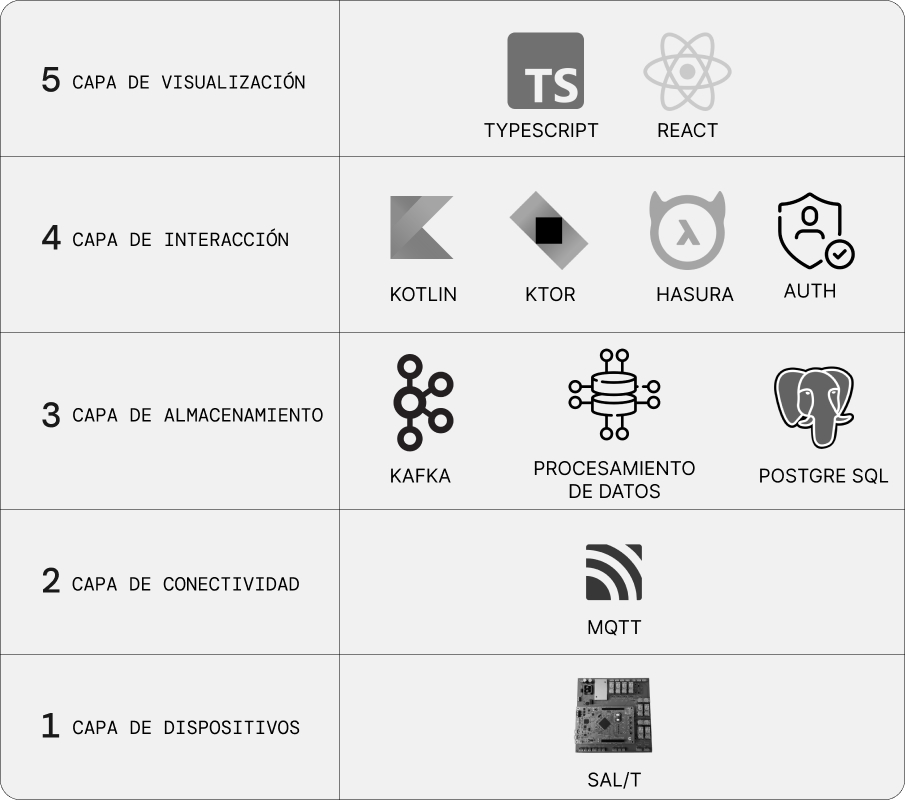
\includegraphics[width=.75\textwidth]{Figures/cuadro.jpg}
  \caption{Arquitectura de la Central Operativa SAL/T.}
  \label{fig:diagBloques}
\end{figure}


\newpage
\subsection{Tecnologías del \textit{front-end}}

\subsubsection{TypeScript}

TypeScript \citep{typescript} es una extensión de código abierto de JavaScript que agrega tipos estáticos opcionales y características de programación orientada a objetos avanzadas, lo que permite una mayor seguridad y mantenibilidad en el código. 


\subsubsection{React}

React \citep{react} es una biblioteca de JavaScript para construir UI reutilizables e interactivas, desarrollada por Facebook y ampliamente utilizada en el desarrollo web. Utiliza un enfoque basado en componentes y el DOM virtual para mejorar el rendimiento y es altamente integrable con otras bibliotecas y frameworks.


\subsubsection{Parcel}

Parcel \citep{parcel} es una herramienta de construcción de código abierto con una estrategia de "cero configuración" que optimiza y empaqueta módulos de JavaScript y otros archivos. En particular, mejora significativamente el flujo de trabajo del desarrollador al ser rápido, fácil de usar y altamente personalizable.


\subsubsection{Apollo GraphQL}

Apollo GraphQL \citep{apollo-graphql} es una plataforma de código abierto para el desarrollo de aplicaciones GraphQL, con una amplia gama de herramientas y servicios para construir y mantener aplicaciones GraphQL de manera efectiva, ofreciendo una administración de caché y una amplia compatibilidad con diferentes frameworks y tecnologías.


\subsubsection{Material UI}

Material UI \citep{material-ui} es una biblioteca de componentes de interfaz de usuario de código abierto basada en Material Design de Google, que ofrece componentes preconstruidos altamente personalizados y una amplia compatibilidad con diferentes tecnologías y frameworks para construir aplicaciones web modernas y atractivas.


\subsubsection{JWT Decode}

JWT Decode \citep{jwt-decode} es una biblioteca JavaScript que decodifica tokens JWT, con características útiles como validación de tokens y verificación de firma. Se integra fácilmente en diferentes frameworks de JavaScript como React y Angular.


%----------------------------------------------------------------------------------------
\newpage
\subsection{Tecnologías del \textit{backend}}


\subsubsection{Kotlin}

Kotlin \citep{kotlin} es un lenguaje de programación de tipado estático que puede correr sobre la máquina virtual de Java y ser compilado en JavaScript y LLVM. También ofrece interoperabilidad con Java, programación funcional, orientación a objetos y manejo de nulos seguro, lo que ha llevado a su popularidad debido a su facilidad de uso y legibilidad.


\subsubsection{Ktor}

Ktor \citep{ktor} es un framework web de Kotlin que permite crear aplicaciones web y API REST de manera fácil y eficiente, con un enfoque en la programación funcional. Ktor es altamente modular y personalizable, lo que significa que los desarrolladores pueden seleccionar solo los componentes que necesitan para su aplicación, reduciendo así la complejidad y el tamaño del código. 


\subsubsection{Kafka}

Kafka \citep{kafka} es una plataforma de streaming de datos que permite a las aplicaciones enviar y recibir datos en tiempo real. Basada en el modelo de publicación/suscripción, se caracteriza por su alta velocidad y rendimiento, haciéndola ideal para aplicaciones que necesitan procesar grandes cantidades de datos en tiempo real.


\subsubsection{Hasura}

Hasura \citep{hasura} es una plataforma sin servidor que permite a los desarrolladores crear y escalar aplicaciones con GraphQL rápidamente. Ofrece seguridad de extremo a extremo y se integra fácilmente con diferentes bases de datos, generando automáticamente una API de GraphQL.


\subsubsection{PostgreSQL}

PostgreSQL \citep{postgresql} es un sistema de gestión de bases de datos de código abierto y gratuito, conocido por su fiabilidad, escalabilidad y seguridad. Ofrece soporte para transacciones ACID, integración con lenguajes de programación populares y una amplia variedad de herramientas y extensiones.


\subsubsection{Mosquitto Broker}

Mosquitto \citep{mosquitto} es un broker MQTT de código abierto utilizado en IoT para transmitir mensajes entre dispositivos. Es popular por su escalabilidad, facilidad de uso y características de seguridad.


%----------------------------------------------------------------------------------------
\newpage
\subsection{Tecnologías del \textit{firmware}}


\subsubsection{C lang}

C \citep{c-lang} es un lenguaje de programación estructurado y de propósito general, ampliamente utilizado en sistemas operativos, aplicaciones de bajo nivel y dispositivos embebidos. Su sintaxis simple y directa permite escribir código claro y legible, y ofrece gran control sobre la memoria y acceso directo al hardware.


\subsubsection{FreeRTOS}

FreeRTOS \citep{free-rtos} es un RTOS de código abierto y gratuito que controla sistemas embebidos y microcontroladores, utilizado en control industrial, automoción y electrónica de consumo, con capacidad de rendimiento confiable y predecible. Es altamente portátil y ofrece gestión de tareas, semáforos, colas y temporizadores para sistemas complejos y eficientes en recursos.


\subsubsection{Paho MQTT \textit{client}}

Paho \citep{paho-mqtt} es una biblioteca cliente MQTT de código abierto que se utiliza para conectar aplicaciones a un broker MQTT. Paho es compatible con una amplia variedad de plataformas y lenguajes de programación, y ofrece una API sencilla para publicar y suscribir mensajes. Es ampliamente utilizado en aplicaciones de IoT y M2M para la transmisión eficiente de datos.


%----------------------------------------------------------------------------------------
\subsection{Herramientas utilizadas}


\subsubsection{Docker}

Docker \citep{docker} es una plataforma de software que permite a los desarrolladores crear, desplegar y ejecutar aplicaciones en contenedores. Estos contenedores permiten que las aplicaciones se ejecuten de manera aislada del sistema operativo y otras aplicaciones, lo que facilita su portabilidad y escalabilidad. 


\subsubsection{Docker Compose}

Docker Compose \citep{docker-compose} es una herramienta que permite definir y ejecutar aplicaciones de múltiples contenedores Docker. Permite a los desarrolladores especificar los servicios y la configuración de cada contenedor en un archivo YAML para simplificar la creación, ejecución y gestión de aplicaciones complejas. 


\subsubsection{Redpanda}

Redpanda \citep{redpanda} es una plataforma de streaming de datos distribuida y de alto rendimiento que combina las funcionalidades de Kafka y Redis. Es una solución escalable y confiable para el procesamiento de datos en tiempo real en entornos empresariales, y es compatible con una amplia variedad de casos de uso, desde el análisis de datos hasta la inteligencia artificial y el aprendizaje automático.


\subsubsection{Git}

Git \citep{git} es un sistema de control de versiones distribuido que se utiliza para rastrear los cambios en el código fuente de un proyecto de software. Permite a los desarrolladores trabajar en colaboración en el mismo código fuente y hacer un seguimiento de las diferentes versiones y ramas del proyecto. 


\subsubsection{MQTT.fx}

MQTT.fx \citep{mqtt-fx} es una herramienta de escritorio de código abierto que se utiliza para probar y depurar conexiones MQTT. Ofrece una interfaz gráfica de usuario fácil de usar para interactuar con brokers MQTT y suscribirse a temas y mensajes. MQTT.fx es compatible con una variedad de características de seguridad, como TLS/SSL y autenticación, lo que lo hace adecuado para su uso en entornos de producción.


\subsubsection{CLion}

CLion \citep{clion} es un entorno de desarrollo integrado (IDE) para programar en C y C++, que ofrece herramientas para la edición de código, depuración, refactorización y gestión de proyectos. Es conocido por su alta capacidad de análisis estático de código, lo que permite a los desarrolladores encontrar errores de forma eficiente.


\subsubsection{Wireshark}

Wireshark \citep{wireshark} es una herramienta de análisis de redes de código abierto y gratuita, utilizada para capturar y analizar paquetes de datos en tiempo real. Permite examinar el tráfico de red para identificar problemas de rendimiento, seguridad y configuración, y es compatible con una amplia variedad de protocolos de red.


\subsubsection{Herramientas del navegador de internet}

Las herramientas del navegador de Internet son características incorporadas en los navegadores web que permiten a los usuarios analizar y modificar elementos de una página web, como su estructura HTML, CSS y JavaScript. Algunas herramientas comunes incluyen la consola de desarrollador, el inspector de elementos, el depurador de JavaScript y el analizador de red, que ayudan a los desarrolladores a depurar problemas y mejorar la calidad de sus sitios web.


\subsubsection{JTAG}

JTAG (Joint Test Action Group) \citep{jtag} es un estándar para la depuración y programación de dispositivos electrónicos. Permite acceder a los pines de prueba de un dispositivo para realizar pruebas de hardware y depuración a nivel de circuito. JTAG se ha convertido en un estándar común para la depuración y programación de dispositivos, y muchas herramientas de desarrollo de software y hardware lo admiten.


\subsubsection{ST-Link}

ST-Link \citep{st-link} es una herramienta de programación y depuración de microcontroladores fabricada por STMicroelectronics. Se utiliza para programar y depurar microcontroladores STM32 y otros dispositivos compatibles con JTAG o SWD. La herramienta se conecta al ordenador mediante USB y se puede usar con una variedad de entornos de desarrollo integrados (IDE) y herramientas de depuración. 


\subsubsection{STM32CubeMX}

STM32CubeMX \citep{stm32-cubemx} es una herramienta de configuración gráfica para dispositivos STM32 que permite a los desarrolladores generar automáticamente código inicial para su proyecto. Ofrece una interfaz de usuario intuitiva que simplifica la configuración de periféricos y pines, y admite una variedad de opciones de generación de código. 


\subsubsection{STM32CubeProgrammer}

STM32CubeProgrammer \citep{stm32-cubeprogrammer} es una herramienta de programación y actualización de firmware para dispositivos STM32 que permite programar y depurar dispositivos STM32, así como actualizar su firmware en campo. Es compatible con una variedad de interfaces de programación, como JTAG, SWD y UART, y es fácil de usar gracias a su interfaz gráfica de usuario. 



